%%%%%%%%%%%%%%%%%%%%%%%%%%%%%%%%%%%%%%%%%%%%%%%%%%%%%%%%%%%%%%%%%%%%%%%%%%%%%%%%%%
\begin{frame}[fragile]\frametitle{}
\begin{center}
{\Large Types and Paths of Yogic Traditions}
\end{center}
\end{frame}


%%%%%%%%%%%%%%%%%%%%%%%%%%%%%%%%%%%%%%%%%%%%%%%%%%%%%%%%%%%
\begin{frame}[fragile]\frametitle{Current Traditions of Yoga}
Just as there are many definitions of yoga, there are many types of yoga as well. 

\tiny{(Ref: An Ultimate Guide to 15 Most Popular Types of Yoga - Naveen Sharma ashmayuyoga.com)}
\end{frame}

%%%%%%%%%%%%%%%%%%%%%%%%%%%%%%%%%%%%%%%%%%%%%%%%%%%%%%%%%%%
\begin{frame}[fragile]\frametitle{Hath Yog(हठ योग)}
	\begin{itemize}
	\item One of the oldest and traditional forms of Yoga
	\item Refers to a practice that combines poses, or asanas, with breathing techniques
	\item Asks to first purify our physical body before higher practices like meditations
	\item Emphasizes on holding the Asana for a longer time with a complete awareness of the body and breath. The pace of the class is slow
	\item Is for a beginner Student
	\end{itemize}

\begin{center}
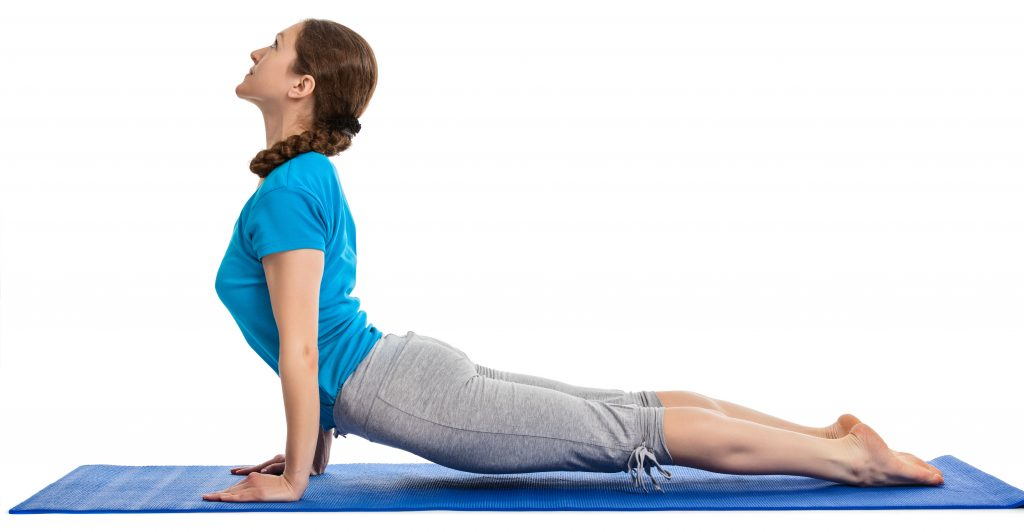
\includegraphics[width=0.6\linewidth,keepaspectratio]{yog1}

\tiny{(Ref: An Ultimate Guide to 15 Most Popular Types of Yoga - Naveen Sharma ashmayuyoga.com)}
\end{center}

\end{frame}

%%%%%%%%%%%%%%%%%%%%%%%%%%%%%%%%%%%%%%%%%%%%%%%%%%%%%%%%%%%
\begin{frame}[fragile]\frametitle{Ashtang Yog (अष्टांग योग)}
	\begin{itemize}
	\item Created by one of the greatest sages Patanjali
	\item Ashtang Vinyasa is popularized by Sri K. Pattabhi Jois. Consists of six series and all the series have asana which is practiced in vinyasa keeping breath, alignment, bandha, drishti in mind.
	\item Quite challenging.
	\item Two approaches:
	\begin{itemize}
	\item Teacher gives instructions about every pose
	\item Students practise on their own and the teacher only comes and corrects if required (Mysore style)
	
	\end{itemize}
	\end{itemize}

\begin{center}
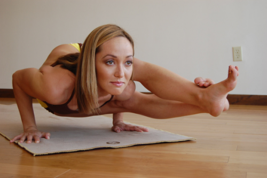
\includegraphics[width=0.5\linewidth,keepaspectratio]{yog21}

\tiny{(Ref: An Ultimate Guide to 15 Most Popular Types of Yoga - Naveen Sharma ashmayuyoga.com)}
\end{center}

\end{frame}

%%%%%%%%%%%%%%%%%%%%%%%%%%%%%%%%%%%%%%%%%%%%%%%%%%%%%%%%%%%
\begin{frame}[fragile]\frametitle{Vinyasa Yog(विन्यास योग)}

	\begin{itemize}
	\item Faster pased, requires you to move continuously throughout the class
	\item To learn how to quickly move from one posture to another with ease, just like dance
	\item To connect each movement with breath
	\end{itemize}

\begin{center}
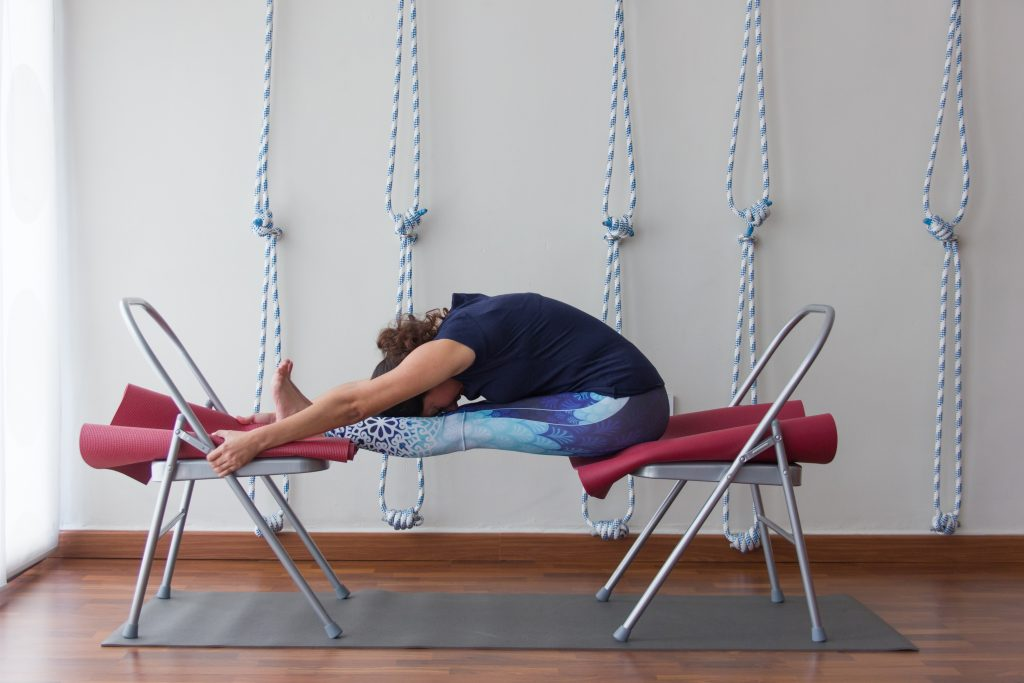
\includegraphics[width=0.6\linewidth,keepaspectratio]{yog3}

\tiny{(Ref: An Ultimate Guide to 15 Most Popular Types of Yoga - Naveen Sharma ashmayuyoga.com)}
\end{center}

\end{frame}

%%%%%%%%%%%%%%%%%%%%%%%%%%%%%%%%%%%%%%%%%%%%%%%%%%%%%%%%%%%
\begin{frame}[fragile]\frametitle{Iyengar Yog(अयंगार योग)}
	\begin{itemize}
	\item Named after BKS Iyengar
	\item Emphasizes on the detailed instructions, precision and alignment of the asana with an in-depth awareness of breath
	\item Is practised with props like ropes, straps, blocks, bolsters, chairs, tables etc
	\end{itemize}

\begin{center}
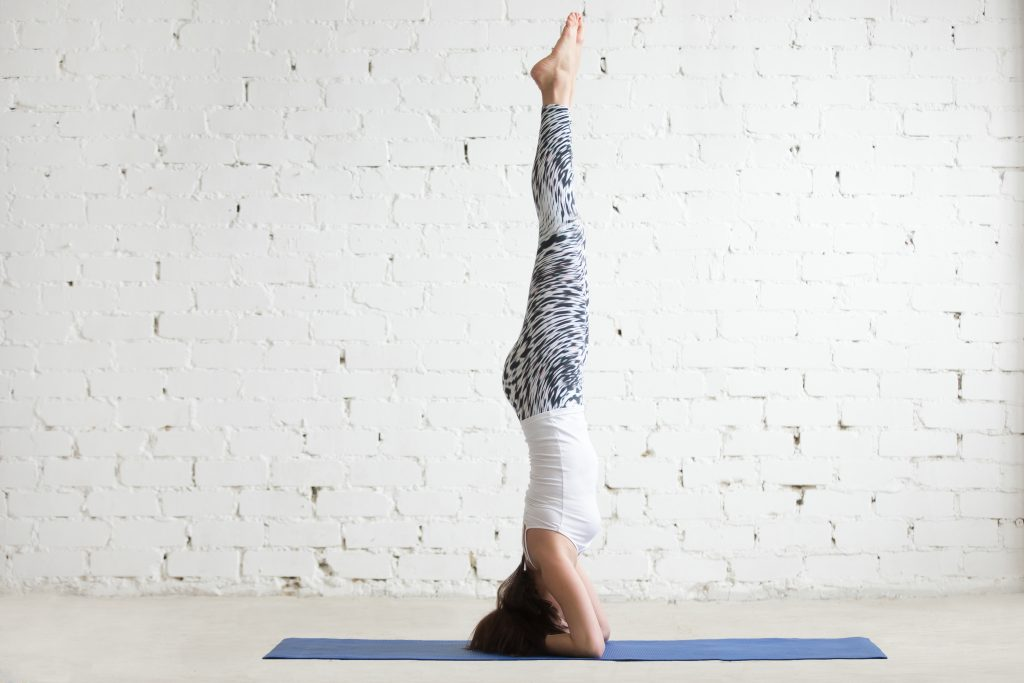
\includegraphics[width=0.6\linewidth,keepaspectratio]{yog4}

\tiny{(Ref: An Ultimate Guide to 15 Most Popular Types of Yoga - Naveen Sharma ashmayuyoga.com)}
\end{center}

\end{frame}

%%%%%%%%%%%%%%%%%%%%%%%%%%%%%%%%%%%%%%%%%%%%%%%%%%%%%%%%%%%
\begin{frame}[fragile]\frametitle{Shivanand Yog(शिवानन्द योग)}
	\begin{itemize}
	\item Has 12 basic asanas, for anyone to perform
	\item Focuses on preserving health and wellness of the students. 
	\item Emphasizes mainly on breathing, relaxation, diet, exercise and positive thinking.
	\end{itemize}

\begin{center}
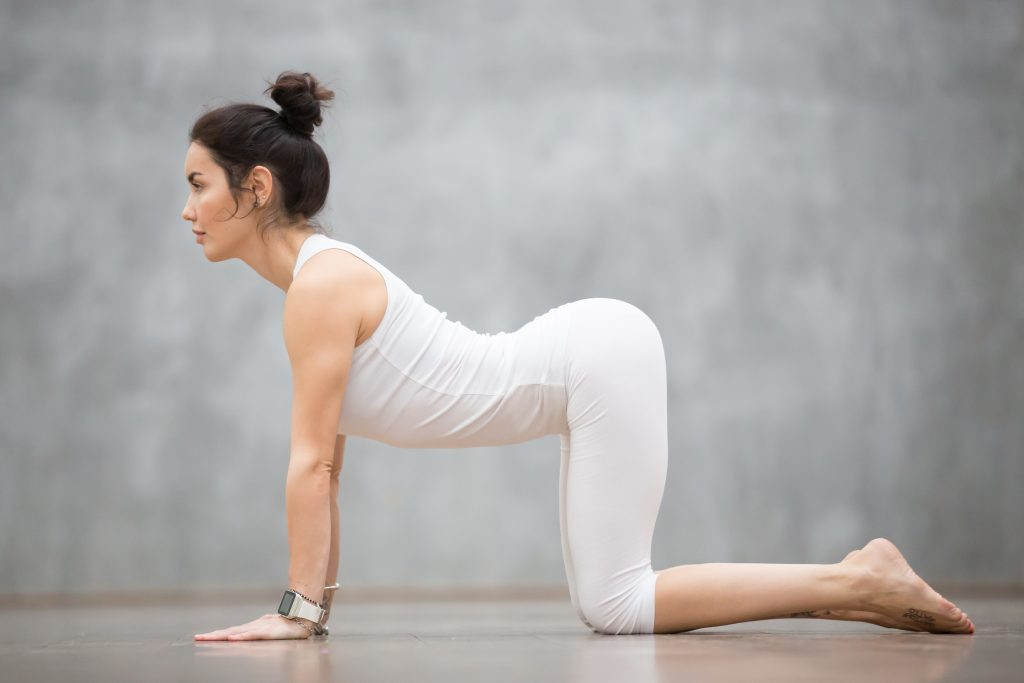
\includegraphics[width=0.6\linewidth,keepaspectratio]{yog5}

\tiny{(Ref: An Ultimate Guide to 15 Most Popular Types of Yoga - Naveen Sharma ashmayuyoga.com)}
\end{center}

\end{frame}

%%%%%%%%%%%%%%%%%%%%%%%%%%%%%%%%%%%%%%%%%%%%%%%%%%%%%%%%%%%
\begin{frame}[fragile]\frametitle{Satyanand Yog(सत्यानन्द योग)}
	\begin{itemize}
	\item Developed by Swami Satyananda Saraswati
	\item Involves the practice of Asana, Pranayama, Shatkarmas, Yoga Nidra, Kriya Yoga, Kundalini Yoga, Mudras, Bandhas, Meditation, Chanting, Karma yoga etc.
	\end{itemize}

\begin{center}
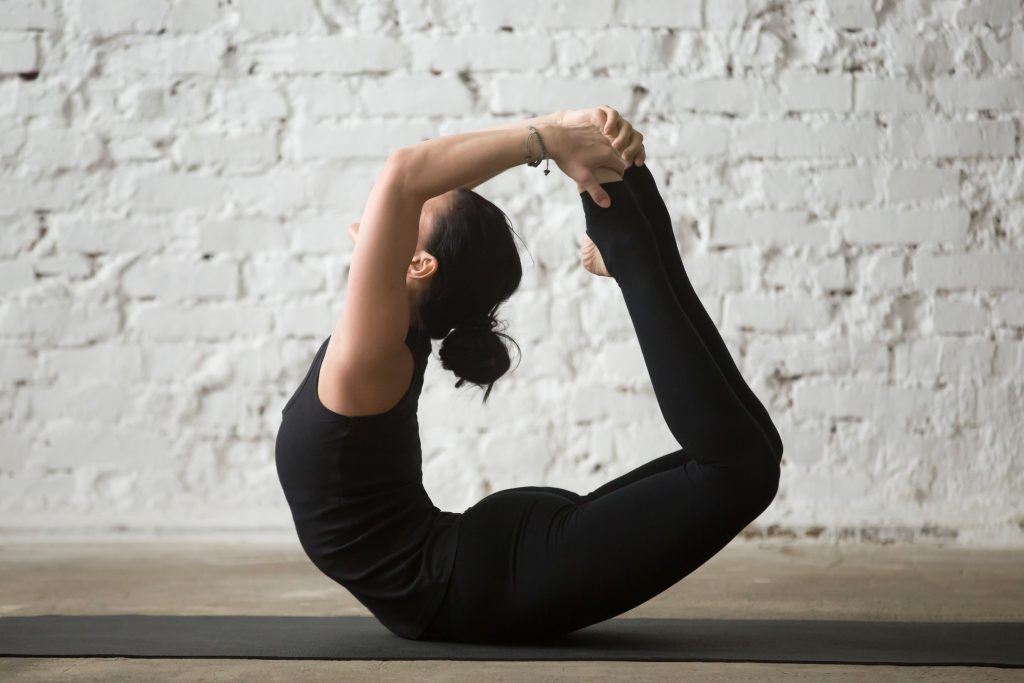
\includegraphics[width=0.6\linewidth,keepaspectratio]{yog6}

\tiny{(Ref: An Ultimate Guide to 15 Most Popular Types of Yoga - Naveen Sharma ashmayuyoga.com)}
\end{center}

\end{frame}

%%%%%%%%%%%%%%%%%%%%%%%%%%%%%%%%%%%%%%%%%%%%%%%%%%%%%%%%%%%
\begin{frame}[fragile]\frametitle{Bikram Yog(बिक्रम योग)}
	\begin{itemize}
	\item Developed by Bikram Choudhury
	\item Consists of 26 postures in set cycles over a 90-minute class
	\item Classes happen in a heated room with temperature in between 35–42 C (95–108 F) with a humidity of 40\%
	\end{itemize}

\begin{center}
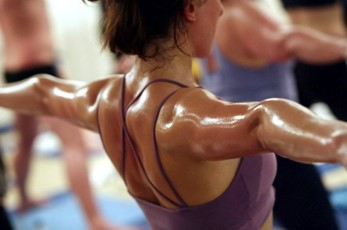
\includegraphics[width=0.4\linewidth,keepaspectratio]{yog19}

\tiny{(Ref: An Ultimate Guide to 15 Most Popular Types of Yoga - ashmayuyoga.com)}
\end{center}

\end{frame}

%%%%%%%%%%%%%%%%%%%%%%%%%%%%%%%%%%%%%%%%%%%%%%%%%%%%%%%%%%%
\begin{frame}[fragile]\frametitle{Kundalini Yog(कुण्डलिनि योग)}
	\begin{itemize}
	\item Quite different from the regular Yoga
	\item You practice postures, pranayama, and meditation and along with it you also perform chanting and singing. 
	\item Average session: 50\% exercise, 20\% breath work, 20\% meditation, and 10\% relaxation
	\item It is all about releasing the coiled (kundalini) energy stored within you.
	\end{itemize}

\begin{center}
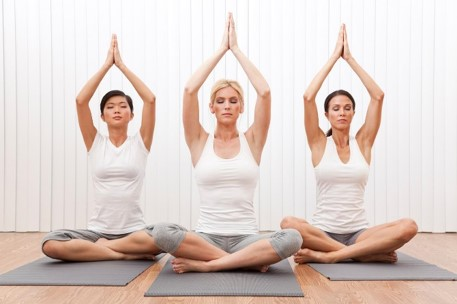
\includegraphics[width=0.6\linewidth,keepaspectratio]{yog20}

\tiny{(Ref: An Ultimate Guide to 15 Most Popular Types of Yoga - Naveen Sharma ashmayuyoga.com)}
\end{center}

\end{frame}

%%%%%%%%%%%%%%%%%%%%%%%%%%%%%%%%%%%%%%%%%%%%%%%%%%%%%%%%%%%
\begin{frame}[fragile]\frametitle{Yin Yog(यिन योग)}
	\begin{itemize}
	\item Is a slow-paced style of yoga practice, need to hold the asanas for longer periods of time
	\item The props are used to reduce your body strain and you perform without actually putting pressure on the muscles.
	\end{itemize}

\begin{center}
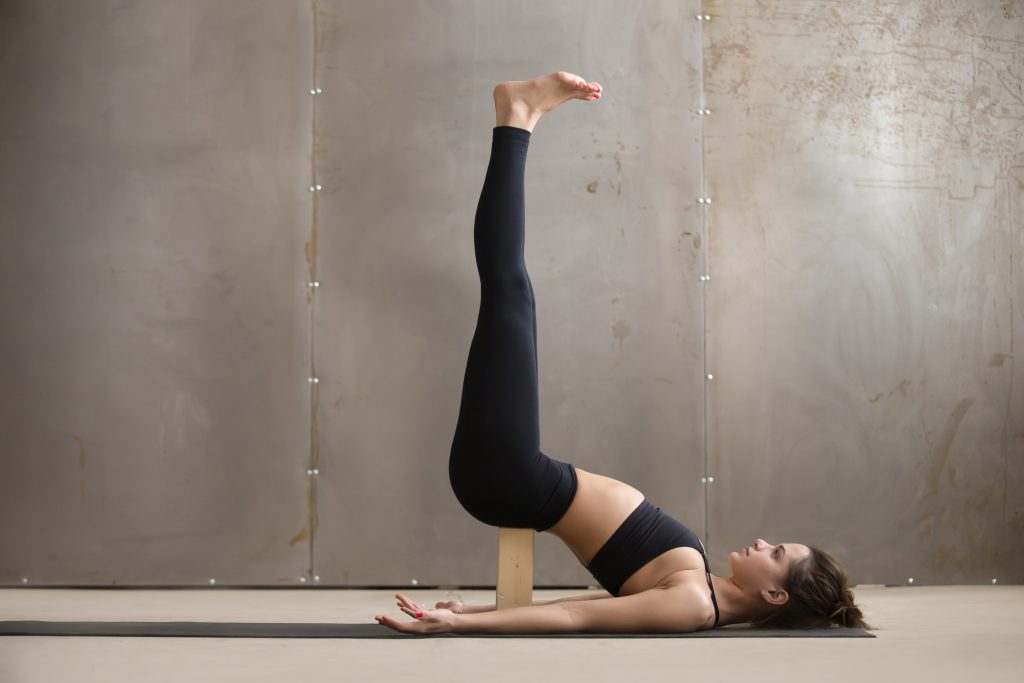
\includegraphics[width=0.6\linewidth,keepaspectratio]{yog9}

\tiny{(Ref: An Ultimate Guide to 15 Most Popular Types of Yoga - Naveen Sharma ashmayuyoga.com)}
\end{center}

\end{frame}


%%%%%%%%%%%%%%%%%%%%%%%%%%%%%%%%%%%%%%%%%%%%%%%%%%%%%%%%%%%
\begin{frame}[fragile]\frametitle{Restorative Yog}
	\begin{itemize}
	\item Focuses more on relaxation, calming the mind, and healing the body
	\item Emphasizes of this form is on helping people to recover from their injuries
	\end{itemize}

\begin{center}
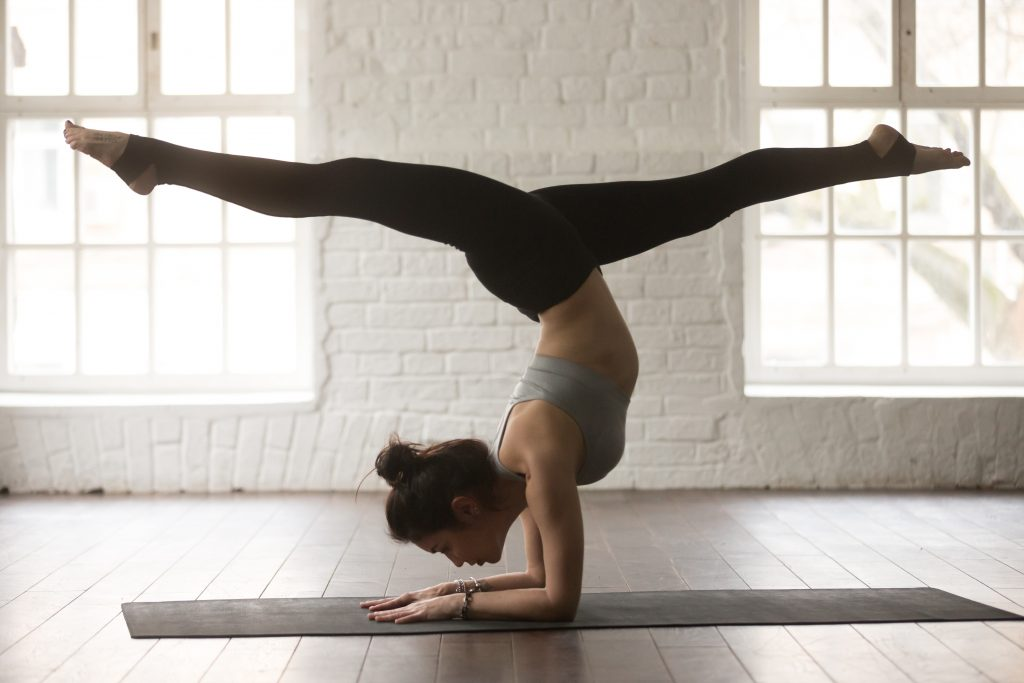
\includegraphics[width=0.6\linewidth,keepaspectratio]{yog10}

\tiny{(Ref: An Ultimate Guide to 15 Most Popular Types of Yoga - Naveen Sharma ashmayuyoga.com)}
\end{center}

\end{frame}

%%%%%%%%%%%%%%%%%%%%%%%%%%%%%%%%%%%%%%%%%%%%%%%%%%%%%%%%%%%
\begin{frame}[fragile]\frametitle{Power Yog}
	\begin{itemize}
	\item Is a very vigorous and fitness-based approach to vinyasa yoga
	\item Designed to model Ashtanga Vinyasa Yoga practice keeping it more flexible wherein the teachers can choose what poses they want to add to the flow
	\end{itemize}

\begin{center}
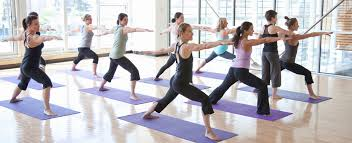
\includegraphics[width=0.6\linewidth,keepaspectratio]{yog14}

\tiny{(Ref: Workshops \& Events - The Healing Lily)}
\end{center}

\end{frame}

%%%%%%%%%%%%%%%%%%%%%%%%%%%%%%%%%%%%%%%%%%%%%%%%%%%%%%%%%%%
\begin{frame}[fragile]\frametitle{AntiGravity Yog}
	\begin{itemize}
	\item Is created by Cristopher Harrison
	\item Uses a silk hammocks to practice all the poses
	\item Supports the students in all the poses, help them deepen the stretches with very less or no strain
	\item Is to remove compression from the spine and improve spinal health.
	\end{itemize}

\begin{center}
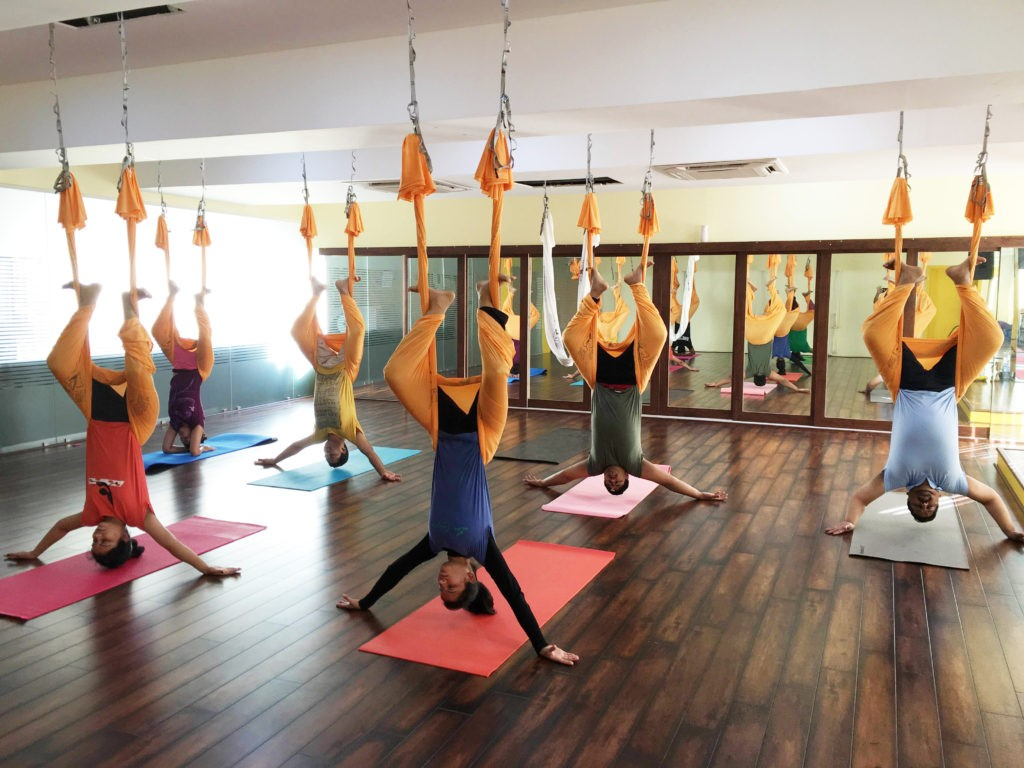
\includegraphics[width=0.6\linewidth,keepaspectratio]{yog11}

\tiny{(Ref: An Ultimate Guide to 15 Most Popular Types of Yoga - Naveen Sharma ashmayuyoga.com)}
\end{center}
\end{frame}


%%%%%%%%%%%%%%%%%%%%%%%%%%%%%%%%%%%%%%%%%%%%%%%%%%%%%%%%%%%
\begin{frame}[fragile]\frametitle{Acro Yog}
	\begin{itemize}
	\item Brings together the principle of Hatha Yoga, Vinyasa Yoga, Acrobatics, Healing and Massage Techniques
	\item You would need a partner 
	\item Build a great amount of strength and improve flexibility.
	\end{itemize}

\begin{center}
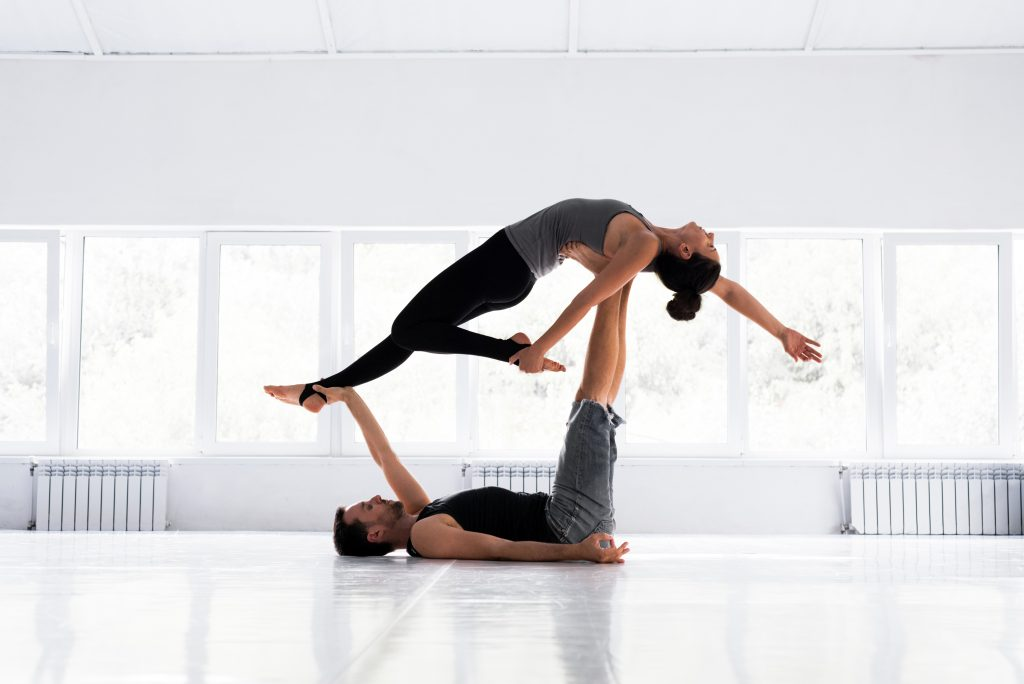
\includegraphics[width=0.6\linewidth,keepaspectratio]{yog12}

\tiny{(Ref: An Ultimate Guide to 15 Most Popular Types of Yoga - Naveen Sharma ashmayuyoga.com)}
\end{center}
\end{frame}

%%%%%%%%%%%%%%%%%%%%%%%%%%%%%%%%%%%%%%%%%%%%%%%%%%%%%%%%%%%
\begin{frame}[fragile]\frametitle{Kripalu Yog (कृपालु योग)}
	\begin{itemize}
	\item Balanced focus on the mind, body, and spirit.
	\item Very gentle and soothing
	\item Helps you learn your own abilities and allows you to look inward
	\end{itemize}

\begin{center}
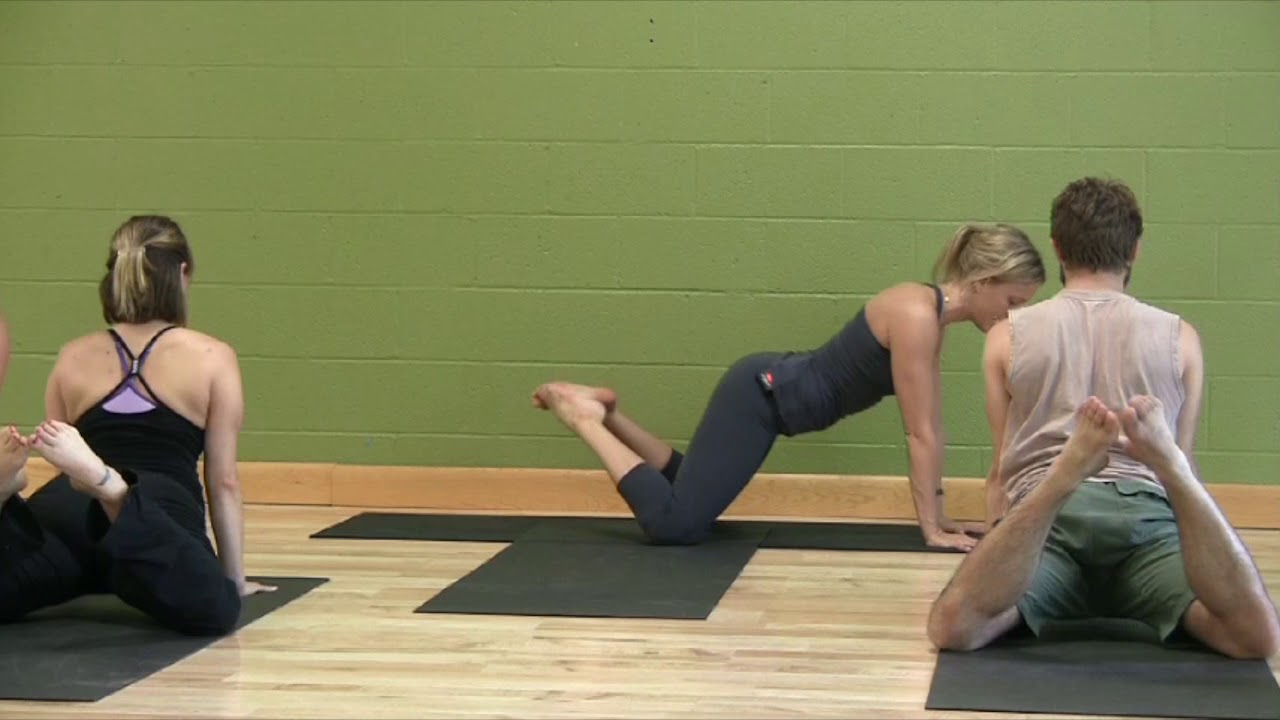
\includegraphics[width=0.6\linewidth,keepaspectratio]{yog13}

\tiny{(Ref: Moderate Kripalu Yoga Vinyasa Flow Class with Coby Kozlowski)}
\end{center}

\end{frame}
